\documentclass[12pt, letterpaper]{article}
\usepackage{graphicx} % Required for inserting images
\setlength{\parskip}{.8em}
\setlength{\parindent}{2em}

\title{Credit Card Fraud Detection}
\author{Huy Pham}
\date{October 2024}
\begin{document}

\maketitle

\section{Introduction}
    \subsection{Project Motivation}
        In 2021, the Federal Trade Commission (FTC) received nearly 390,000 reports of credit card fraud, making it one of the most common types of fraud in the United States. This issue is projected to result in losses totaling \$165.1 billion over the next decade. Given the significant impact on society, leveraging machine learning technology to address this problem is increasingly beneficial.

    \subsection{Objective}
        In this project, our primary goal is to develop a reliable machine learning model to detect fraudulent credit card transactions. This involves a thorough analysis of the dataset to understand its distributions and engineering the most suitable model that captures the relationship between the target variable and features. We utilize Python libraries like Scikit-learn, Matplotlib, Numpy, and Pandas for implementation and visualization. The dataset used for this project was sourced from Kaggle. However, it is also important to note that this is an introductory project to machine learning which serves as an educational research project.
        
\section{Dataset Exploratory Analysis}
    \subsection{Origin}
        The dataset was sourced from Kaggle, which was provided during a collaborative research project between Worldline and Machine Learning Group of ULB (Université Libre de Bruxelles) on big data mining and fraud detection. \cite{Kaggle}
        
    \subsection{Dataset Understanding}
        The dataset has 31 predictors, which is quite time-consuming for the training process. Perhaps finding ways to reduce the dataset dimensions would benefit the project as well as the research model better.

        \par It seems that the dataset is sorted chronologically as the transactions happened as time went on. It is sensible to deem that the features "Time" and "Amount" are much less relevant to the desired model as frauds can happen at any time and any magnitude during the day.

        \par There are in total 284,807 transactions or data points in this dataset. It is also learned that the actual fraudulent transactions in this dataset is extremely underrepresented as the mean value for feature Class is extremely close to 0 (meaning there are a lot of 0s and so few 1s). The imbalance of the dataset is heavily concerning as the relationship displayed in this dataset between the two types of data points are not so credible.        

    \subsection{Data Preparation}
        The data types recorded in the dataset features are efficient for computing algorithms, which is beneficial to the training time of the research model. It is also noted that the dataset contains no invalid values (null values).

        \par Duplicates are identified within the dataset, with 1081 instances. However, dropping duplicates might impact the weight the duplicated points has on the dataset. In fact, the representation of positive class within the dataset is 0.173\% and after dropping the duplicates, the percentage goes down to 0.167\%. Even though the difference is negligible in most cases, it is still crucial to have more representation of these fraudulent data points in this extremely skewed dataset. This highlights the relevance of duplicated data points in the dataset to the relationship between two classes.
        
        \begin{figure}[h]
            \centering
            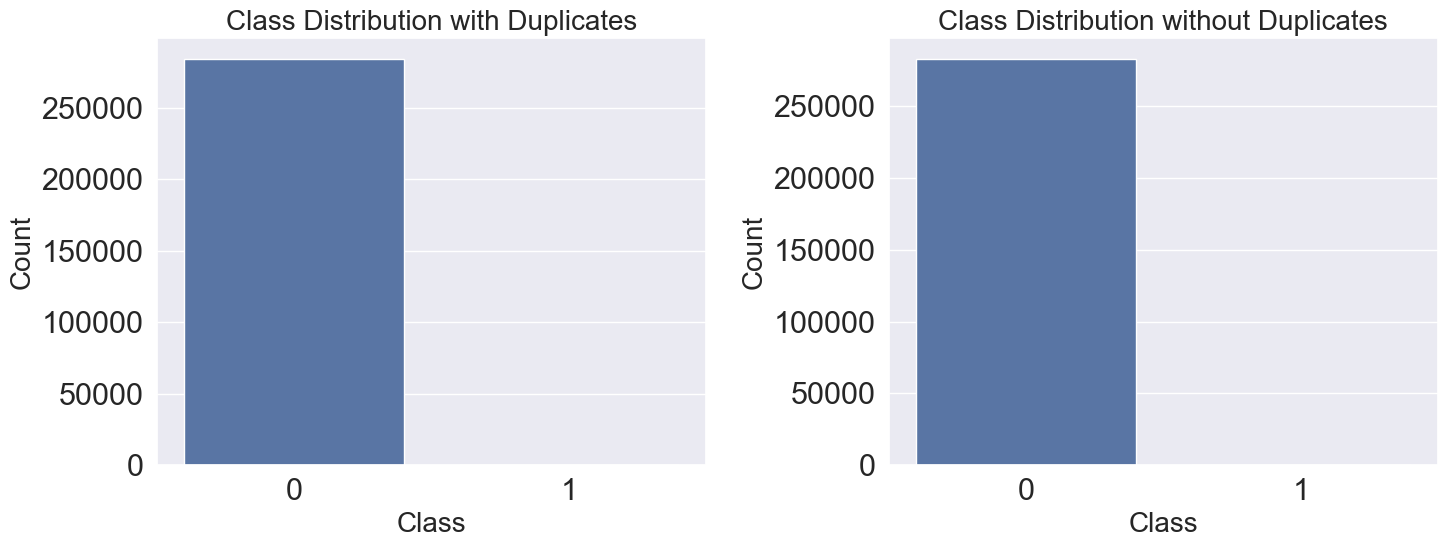
\includegraphics[width=1\linewidth]{Figures/Class-representation.png}
            \caption{Class Distributions Concerning Dataset Duplication}
            \label{fig:enter-label}
        \end{figure}
        
\section{Methodology}
    \subsection{Model Evaluation Metrics}
        Accuracy is highly a biased metric since the dataset is super skewed. Precision provide insights to how accurate is the model predictions of the positive class. Sensitivity display how well the model is able to identify the positive class (i.e. the fraudulent class).

        \par True Positive Rate and False Positive Rates indicates the credibility of the model's prediction. It would portrays the accuracy of each positive/negative prediction, thus, allowing us to pursue further.

        \par F1-score is a particularly helpful metric

        \par ROC-AUC score

        \par Average Precision is also indicative of the model's performance.

    \subsection{Bias and Variance}
        K-fold cross-validation is implemented to ensure bias and variance are not too high, thus, countering over-fitting and under-fitting from happening.

    \subsection{Standardization}
    
    \subsection{Class Weights}
    
    \subsection{Synthetic Minority Over-sampling Technique}
    
    \subsection{Linear Discriminant Analysis}
        
\section{Results}

\section{Conclusion}

\begin{thebibliography} {1}
    \bibitem{Kaggle}
    Machine Learning Group - ULB. “Credit Card Fraud Detection” Kaggle, 2018, www.kaggle.com/datasets/mlg-ulb/creditcardfraud.
    
\end{thebibliography}
    
\end{document}
